%Declaramos la clase de documento
\documentclass[12pt, letterpaper]{article}

%Paquetes de idioma y codificación de caracteres
\usepackage[utf8]{inputenc}
\usepackage[spanish]{babel}

%Otros paquetes
\usepackage{graphicx}

%Dimensiones del Documento
\usepackage[left=2cm,right=2cm,top=2cm,bottom=2cm]{geometry}
\usepackage{graphicx}%para las figuras
\usepackage{float}%para usar [H]
\usepackage{amsmath}
\usepackage{enumerate}%para los enumerados
\usepackage{hyperref}
\renewcommand{\labelitemi}{$-$}
\renewcommand{\labelitemi}{$\cdot$}

%Datos para el titulo de nuestro documento
   %\title{Informe de Laboratorio N°08 - Base de Datos II}
   %\author{Gabriela Atahuachi Rivera}
   %\date{\today}

\begin{document}

%Imprimimos la pagina de titulo
\title{Caratula}

\begin{titlepage}
	\begin{center}
		\large{UNIVERSIDAD PRIVADA DE TACNA}\\

		\vspace*{-0.025in}
			\begin{figure}[htb]
				\begin{center}
					
\includegraphics[width=8cm]{./Imagenes/LogoUpt}
				\end{center}
			\end{figure}

		\vspace*{0.15in}
		INGENIERIA DE SISTEMAS  \\

		\vspace*{0.5in}
			\begin{large}
			TITULO:\\
			\end{large}

		\vspace*{0.1in}
			\begin{large}
				\textbf{Informe de Laboratorio 8} \\
				\textbf{Instalación de un Gestor de Base de Datos Oracle} \\
			\end{large}

		\vspace*{0.3in}
			\begin{large}
				\textbf{CURSO:} \\
			\end{large}

		\vspace*{0.1in}
			\begin{large}
				Base De Datos II \\
			\end{large}

		\vspace*{0.3in}
			\begin{large}
				\textbf{DOCENTE:} \\
			\end{large}

		\vspace*{0.1in}
			\begin{large}
				Ing. Patrick Cuadros Quiroga \\
			\end{large}

		\vspace*{0.2in}
			\vspace*{0.1in}
				\begin{large}
					Integrantes: \\
					\begin{flushleft}
						Atahuachi Rivera, Gabriela Atahuachi	\hfill	(2016055341) \\
					\end{flushleft}
				\end{large}
	\end{center}
\end{titlepage}

\tableofcontents %para el índice
	\thispagestyle{empty} %para el índice sin numero
		\newpage
			\setcounter{page}{1}%reiniciar contador de paginas despues del indice
				\section{Información General}

	\begin{itemize}
		\subsection{Objetivos:}
			\item Descarga e Instalación del Docker Desktop
			\item Poder Configurar Correctamente el Docker Desktop en PowerShell
			\item Poder Instalar Correctamente las Consultas Requeridas
		\subsection{Recursos Utilizados:}
			\item Al menos 4 GB de RAM.
			\item CPU SLAT-capable feature.
			\item Windows 10 64-bit: Pro, Enterprise o Education
			\item Docker Desktop
			\item Oracle SQL Developer for Windows.
		\subsection{Consideraciones Iniciales:}
			\item Tener instalado las opciones de Windows: Hyper-V.
			\item Tener instalado Docker Desktop.
			\item Crear dos carpetas en una unidad donde se pueda modificar datos DATALNX y DATAWIN.
	\end{itemize}
				\section{Procedimientos.}

	\begin{itemize}
		\subsection{Parte 1. Iniciando Docker.}
			\item Abrimos nuestro menú de inicio y buscamos la aplicación Docker for Windows.
				\begin{figure}[htb]
					\begin{center}
						
\includegraphics[width=8cm]{./Imagenes/BuscarDocker}
					\end{center}
				\end{figure}
			\item Una vez iniciado se podrá visualizar el icono de Docker en el área de notificación.
				\begin{figure}[htb]
					\begin{center}
						
\includegraphics[width=6cm]{./Imagenes/VerIcono}
					\end{center}
				\end{figure}
			\item Asimismo se podrá visualizar la ventana de bienvenida.
				\begin{figure}[htb]
					\begin{center}
						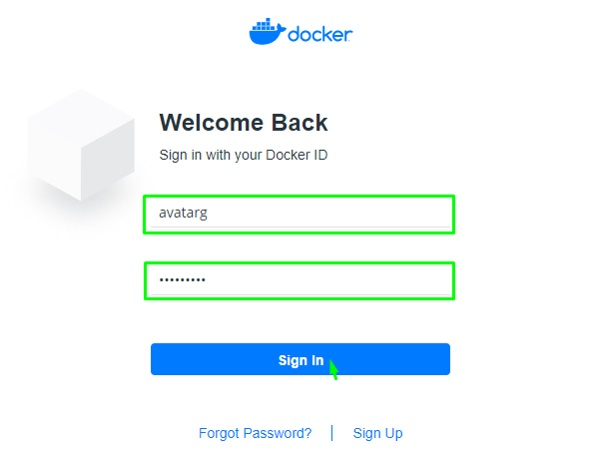
\includegraphics[width=9cm]{./Imagenes/Loguearse}
					\end{center}
				\end{figure}
			\item El resultado sería como se muestra en la siguiente imagen.
					\begin{figure}[htb]
						\begin{center}
							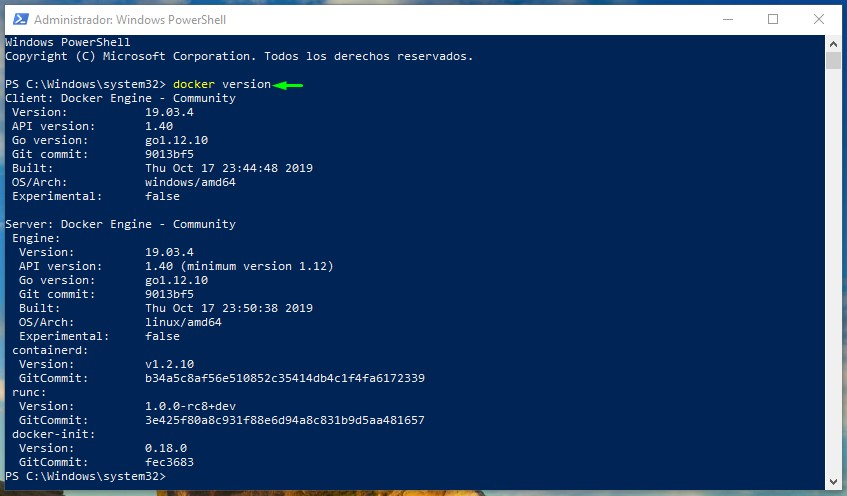
\includegraphics[width=16cm]{./Imagenes/VersionDocker}
						\end{center}
					\end{figure}
				\vspace{7cm}
		\subsection{Parte 2. Ceando un Contenedor son Oracle Database para Linux.}
			\item Ingresamos a Nuestro Buscador de Internet Google Chrome  o cualquier otro.
				\begin{figure}[htb]
					\begin{center}
						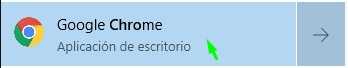
\includegraphics[width=8cm]{./Imagenes/BuscarAppGoogle}
					\end{center}
				\end{figure}
			\item Luego Copiamos y Pegamos el Siguiente Link.
				\begin{center}
					\url{https://hub.docker.com/}
				\end{center}
				\vspace{7cm}
			\item Inciamos Sesión o nos Creamos una Cuante Nueva.
				\begin{figure}[htb]
					\begin{center}
						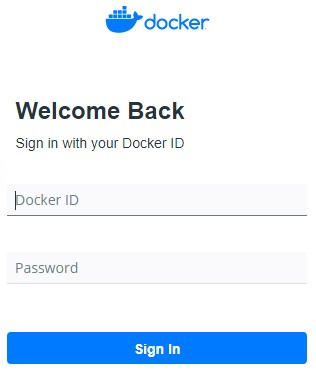
\includegraphics[width=6cm]{./Imagenes/Loguearse3}
					\end{center}
				\end{figure}				
			\item Seguidamente de loguearnos, seleccionamos la caja de texto de busqueda y digitamos lo siguiente:
				\begin{figure}[htb]
					\begin{center}
						
\includegraphics[width=9cm]{./Imagenes/BuscarOracleDatabase1}
					\end{center}
				\end{figure}
			\item Y seleccionamos la Primera Opción, tal y como se muestra en la siguiente imagen.
				\begin{figure}[htb]
					\begin{center}
						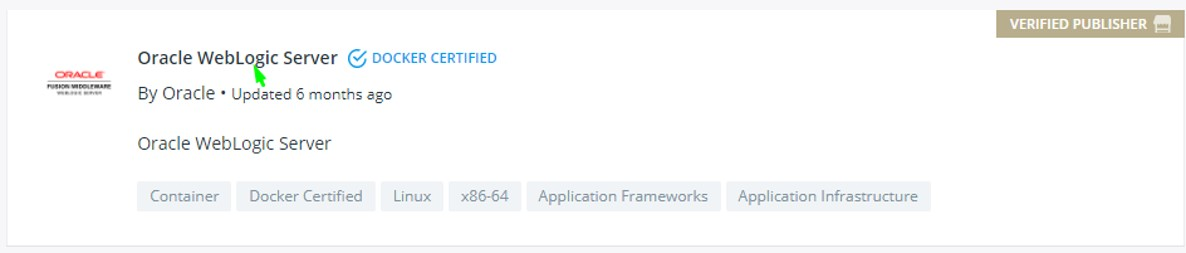
\includegraphics[width=15cm]{./Imagenes/Seleccionar1}
					\end{center}
				\end{figure}
			\item Procedemos con el CheckOut, seleccionando el boton indicado en la imagen.
				\begin{figure}[htb]
					\begin{center}
						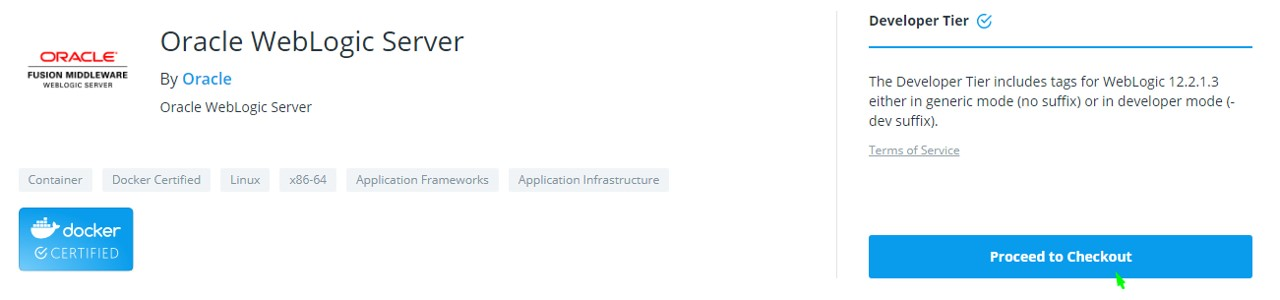
\includegraphics[width=15cm]{./Imagenes/Seleccionar2}
					\end{center}
				\end{figure}
				\vspace{5cm}
			\item Ingresamos las casillas y seleccionamos el boton indicado en la siguiente imagen.
				\begin{figure}[htb]
					\begin{center}
						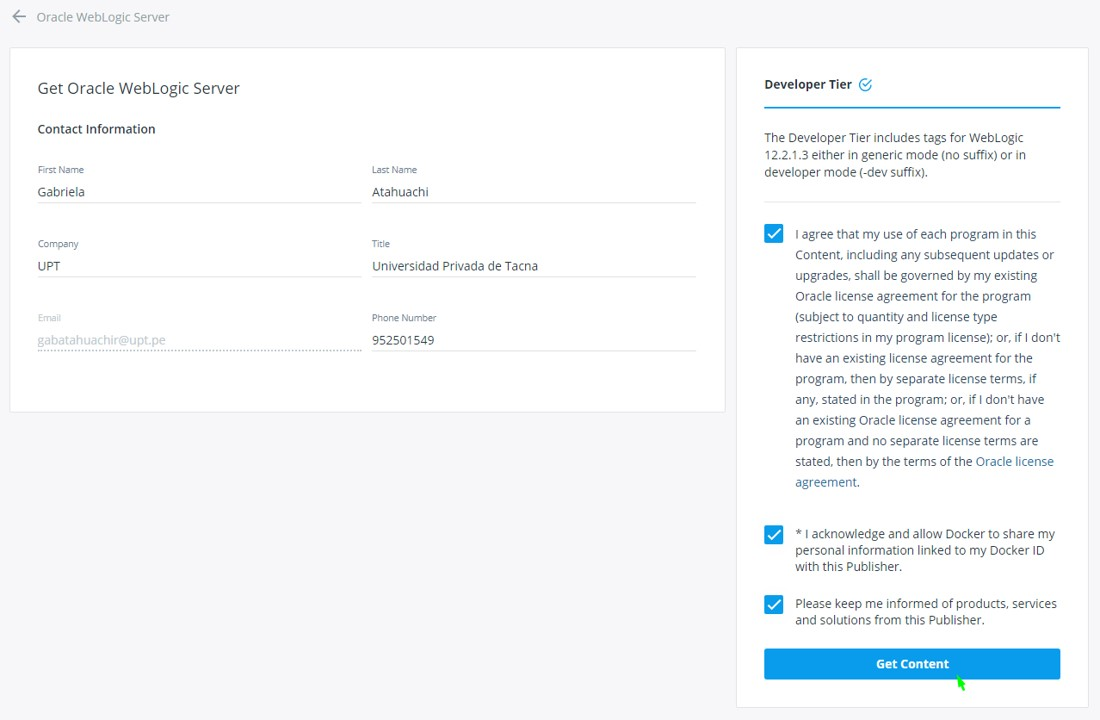
\includegraphics[width=15cm]{./Imagenes/Seleccionar3}
					\end{center}
				\end{figure}
			\item Al final obtenemos el acceso al contenido.
				\begin{figure}[htb]
					\begin{center}
						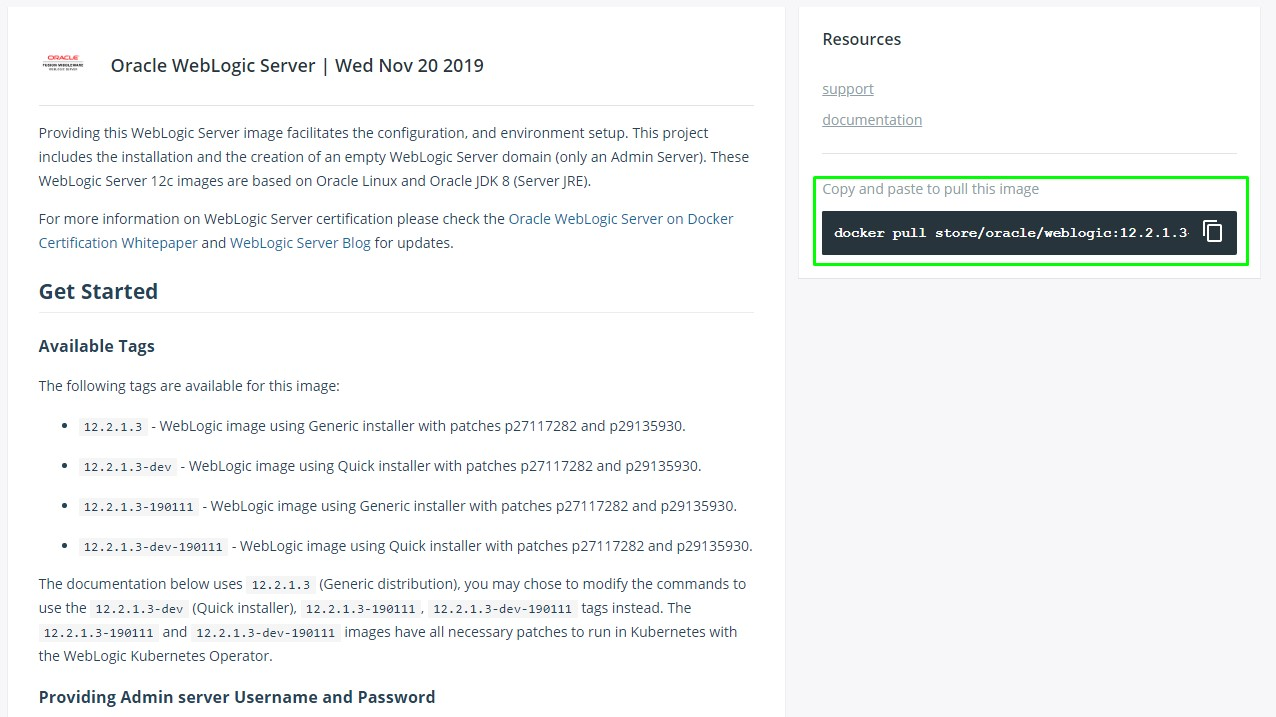
\includegraphics[width=15cm]{./Imagenes/Seleccionar4}
					\end{center}
				\end{figure}
				\vspace{7cm}
			\item Ahora buscamos el programa Windows PowerShell.
					\begin{figure}[htb]
						\begin{center}
							
\includegraphics[width=8cm]{./Imagenes/BuscarPowerShell}
						\end{center}
					\end{figure}
				\item Luego lo ejecutamos como administrador para que no genere problemas luego.
					\begin{figure}[htb]
						\begin{center}
							
\includegraphics[width=6cm]{./Imagenes/EjecutarComoAdministrador}
						\end{center}
					\end{figure}
				\item Se mostrará una ventana como la que se ve en la imagen.
					\begin{figure}[htb]
						\begin{center}
							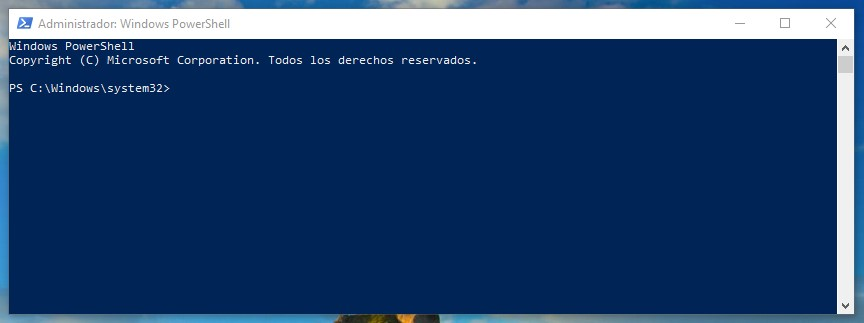
\includegraphics[width=16cm]{./Imagenes/InicioPowerShell}
						\end{center}
					\end{figure}
					\vspace{7cm}
				\item Digitaremos lo siguiente.
					\begin{figure}[htb]
						\begin{center}
							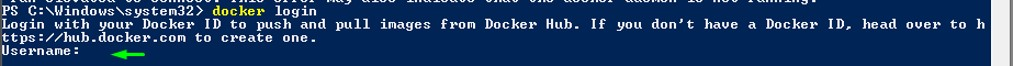
\includegraphics[width=16cm]{./Imagenes/Comando01}
						\end{center}
					\end{figure}
	\end{itemize}
				\include{Secciones/Actividad03}
				\include{Secciones/Actividad04}
				\include{Secciones/Actividad05}
				\include{Secciones/Actividad06}
\end{document}
